\input ../SlidePreamble
\input ../preamble

\begin{document}

{\Huge

  \centerline{\bf TTIC 31230, Fundamentals of Deep Learning}
  \bigskip
  \centerline{David McAllester, April 2017}
\vfill
  \centerline{\bf Deep Reinforcement Learning}
  \vfill
\vfill

\slide{Definition of Reinforcement Learning}

RL is defined by the following properties:

\vfill
\begin{itemize}
\item An environment with {\bf state}.

  \vfill
\item State changes are influenced by {\bf sequential decisions}.

  \vfill
\item  Reward (or loss) depends on {\bf making decisions} that lead to {\bf desirable states}.
\end{itemize}

\slide{Reinforcement Learning Examples}

\begin{itemize}
\item Board games (chess or go)

  \vfill
\item Atari Games (pong)

  \vfill
\item Robot control (driving)

  \vfill
\item Dialog

  \vfill
\item Life

\end{itemize}

\slide{Policies}

A policy is a way of behaving.

\vfill
Formally, a (nondeterministic) policy maps a state to a probability distribution over actions.

\vfill
\begin{eqnarray*}
    \pi(a_t|s_t) & & \mbox{probability of action $a_t$ in state $s_t$}
\end{eqnarray*}

\slide{Imitation Learning}

Construct a training set of state-action pairs $(s,a)$ from experts.

\vfill
Define stochastic policy $\pi_\Phi(s)$.

\vfill
$$\Phi^* = \argmin_\Phi \expectsub{(s,a) \sim \mathrm{Train}}{- \ln \pi_\Phi(a\;|\;s)}$$

\vfill
This is just cross-entropy loss where we think of $a$ as a ``label'' for $s$.

\slide{Dangers of Imperfect Imitation Learning}

Perfect imitation learning would reproduce expert behavior.

Imitation learning is {\bf off-policy} ---
the state distribution in the training data is different from that defined by the policy being learned.

\vfill
Imitating experts, such as expert fire eaters, can be dangersous.  ``Don't try this at home''.

\vfill
Also, imitating experts will never exceed expert performance (consider AlphaZero).

\slide{Markov Decision Processes (MDPs)}

For an RL problem we work with an action policy $\pi$

\vfill
$s_t$ is the state at time $t$

\vfill
$r_t$ is the reward at time $t$

\vfill
$a_t$ is the action taken at time $t$.
\begin{eqnarray*}
  r_t = R(s_t,a_t) & & \mbox{reward at time $t$} \\
  P_T(s_{t+1}|s_t,a_t) & & \mbox{state transition probability}
\end{eqnarray*}

\vfill
The function $R(s,a)$ can allow for a cost of the action $a$.

\vfill
This Data defines a {\bf Markov Decision Process} or {\bf MDP}.

\slide{Optimizing Reward}

In RL we maximize reward rather than minimize loss.

$$\pi^* = \argmax_\pi \;R(\pi)$$

\vfill
$$\begin{array}{rcll}
  R(\pi) & = & \expect{\sum_{t=0}^T \;r_t} &\mbox{episodic reward (go)} \\
\\
& \mbox{or} & \expect{\sum_{t=0}^\infty \;\gamma^t r_t} &\mbox{discounted reward (financial planning)} \\
\\
& \mbox{or} & \lim_{T \rightarrow \infty}\;\frac{1}{T} \;\sum_{t=0}^T \;r_t &\mbox{asymptotic average reward (driving)}
\end{array}$$


\slide{The Value Function}

For discounted reward:

\begin{eqnarray*}
  V^\pi(s) & = & \expect{\sum_t \;\gamma^t r_t  \;\;|\; \pi, \; s_0 = s} \\
  \\
  V^*(s) & = & \sup_\pi \;V^\pi(s) \\
  \\
  \pi^*(a|s) & = & \argmax_a\;\expectsub{s' \sim P_T(s'|s,a)}{V^*(s')} \\
  \\
  V^*(s) & = & \max_a\; R(s,a) + \gamma \expectsub{s' \sim P_T(\cdot|s,a)}{V^*(s')}
\end{eqnarray*}

\slide{Value Iteration}

Suppose the state space and action space are finite.

\vfill
In that case we can do value iteration.

\begin{eqnarray*}
  V_0(s) & = & 0 \\
  \\
  V_{i+1}(s) & = & \max_a\; R(s,a) + \gamma \expectsub{s' \sim P_T(\cdot|s,a)}{V_i(s')}
\end{eqnarray*}

\vfill
If all rewards are non-negative then

$$V_{i+1}(s) \geq V_i(s)\;\;\;\;V_i(s) \leq V^*(s)\;\;\;\;\mathrm{so}\;\lim_{i \rightarrow \infty}\;V_i(s)\;\mathrm{exists}$$

\slide{Value Iteration}

Theorem: {\bf For discounted reward}
\vfill
$$V_\infty(s) \doteq \lim_{i \rightarrow \infty}\;V_i(s) = V^*(s)$$

\slide{Proof}

\begin{eqnarray*}
  \;\Delta & \doteq & \max_s\;\;V^*(s) - V_\infty(s) \\
  \\
  & = & \max_s \left(\begin{array}{l} \max_a R(s,a) + E_{s'|a} \gamma V^*(s') \\ - \max_a R(s,a) + E_{s'|a} \gamma V_\infty(s')\end{array}\right) \\
  \\
    & \leq & \max_s \max_a \left(\begin{array}{l} R(s,a) + E_{s'|a} \gamma V^*(s') \\ - R(s,a) + E_{s'|a} \gamma V_\infty(s')\end{array}\right) \\
  \\
  & = & \max_s \max_a \;E_{s'|a}\; \gamma (V^*(s') - V_\infty(s)) \\
  \\  
  & \leq & \gamma \Delta
\end{eqnarray*}


\slide{The $Q$ Function}

For discounted reward:

\begin{eqnarray*}
  Q^\pi(s,a) & = & E_\pi\;\sum_t \;\gamma^tr_t \;\;|\; \pi, \; s_0 = s,\;a_0 = a \\
  \\
  Q^*(s,a) & = & \sup_\pi \;Q^\pi(s,a) \\
  \\
  \pi^*(a|s) & = & \argmax_a\;Q^*(s,a) \\
  \\
  Q^*(s,a) & = & R(s,a) + \gamma \expectsub{s' \sim P_T(\cdot|s,a)}{\max_{a'}\; Q^*(s',a')}
\end{eqnarray*}

\slide{$Q$-Learning}

We will assume a parameterized $Q$ function $Q_\Phi(s,a)$.
\vfill
{\bf Bellman Error:}
{\huge $$\mathrm{Bell}_\Phi(s,a) \doteq \left(Q_\Phi(s,a) - \left(R(s,a) + \gamma\;\expectsub{s' \sim P_T(s'|s,a)}{\max_{a'}\;Q_\Phi(s',a')}\right)\right)^2$$}

{\bf Theorem}: If $\mathrm{Bell}_\Phi(s,a) = 0$ for all $(s,a)$ then the induced policy is optimal.

\vfill
{\bf Algorithm}: Generate pairs $(s,a)$ from the policy $\argmax_a\;Q_\Phi(s_t,a)$ and repeat
$$\Phi \;\minuseq\; \eta \nabla_\Phi \;\; \mathrm{Bell}_\Phi(s,a)$$


\slide{Issues with $Q$-Learning}

Problem 1: Nearby states in the same run are highly correlated.  This increases the variance of the cumulative gradient updates.

\vfill
Problem 2: SGD on Bellman error tends to be unstable. Failure of $Q_\Phi$ to model unused actions leads to policy change (exploration).
But this causes $Q_\Phi$ to stop modeling the previous actions
which causes the policy to change back ...

\vfill
To address these problems we can use a {\bf replay buffer}.

\slide{Using a Replay Buffer}

We use a replay buffer of tuples $(s_t,a_t,r_t,s_{t+1})$.

\vfill
Repeat:

\vfill
\begin{enumerate}

\item Run the policy $\argmax_a Q_\Phi(s,a)$ to add tuples to the replay buffer.  Remove oldest tuples to maintain a maximum buffer size.

\item {\color{red} $\Psi = \Phi$}
  
\item for $N$ times select a random element of the replay buffer and do
$$\Phi \;\minuseq \; \eta \nabla_\Phi\;(Q_\Phi(s_t,a_t) - (r_t + \gamma \max_{a} Q_{\color{red} \Psi}(s_{t+1},a))^2$$
\end{enumerate}

\slide{Replay is Off-Policy}

Note that the replay buffer is from a {\bf mixture of policies} and is {\bf off-policy} for $\argmax_a\;Q_\Phi(s,a)$.  This seems to be important for stability.

\vfill
This seems related to the issue of stochastic vs. deterministic policies.  More on this later.

\slide{Multi-Step $Q$-learning}

$$\Phi \;\minuseq \;\sum_t \nabla_\Phi \left(Q_\Phi(s_t,a_t) - \sum_{\delta = 0}^{D} \gamma^\delta r_{(t+\delta)}\right)^2$$


\slidetwo{Human-level control through deep RL (DQN)}{Mnih et al., Nature, 2015. (Deep Mind)}
\vfill
We consider a CNN $Q_\Phi(s,a)$.

\vfill
\centerline{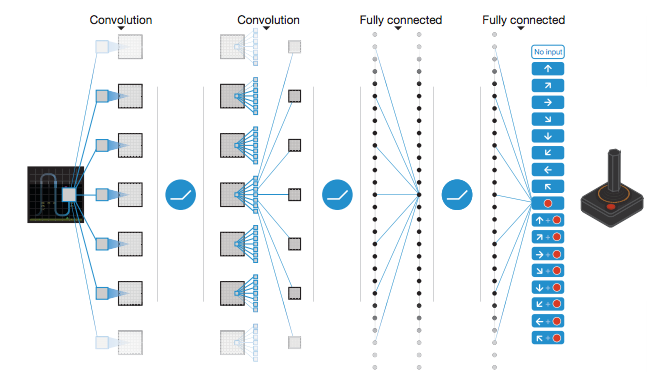
\includegraphics[width=6in]{../images/DQN}}

\slide{Watch The Video}

https://www.youtube.com/watch?v=V1eYniJ0Rnk

\slide{Asynchronous $Q$-Learning (Simplified)}
No replay buffer.
Many asynchronous threads each repeating:
\vfill

  \begin{quotation}
  \noindent $\tilde{\Phi} = \Phi$ (retrieve $\Phi$)\newline \newline
  \noindent using policy $\argmax_a Q_{\tilde{\Phi}}(s,a)$ compute $$s_t,a_t,r_t,\ldots,s_{t+K},a_{t+K},r_{t+K}$$
  \newline
  \noindent {\huge $\Phi \;\minuseq\; \eta \sum_{i=t}^{t+K-D} \nabla_{\tilde{\Phi}}\;\left(Q_{\tilde{\Phi}}(s_i,a_i) - \sum_{\delta = 0}^D \gamma^\delta r_{i+\delta}\right)^2$} (update $\Phi$)
  \end{quotation}

\slide{}
\centerline{\bf The REINFORCE Algorithm}

\vfill
\centerline{\bf Williams, 1992}
\vfill\vfill

\slide{REINFORCE is a Policy Gradient Algorithm}

We assume a parameterized policy $\pi_\Phi(a|s)$.

\vfill
$\pi_\Phi(a|s)$ is normalized while $Q_\Phi(s,a)$ is not.

\slide{Policy Gradient Theorem (Episodic Case)}

$$\Phi^* = \argmax_\Phi\; E_{\pi_\Phi} \; R$$

{\huge
\begin{eqnarray*}
  \nabla_\Phi \;E_{\pi_\Phi}\;R & = & \sum_{s_0,a_0,s_1,a_1,\ldots,s_T,a_T}\;\;\nabla_\Phi P(s_0,a_0,s_1,a_1,\ldots,s_T,a_T)\;R \\
  \\
  \nabla_\Phi \;P(\ldots)R & = & P(S_0){\color{red} \nabla_\Phi \;\pi(a_0)}P(s_1)\pi(a_1) \cdots P(s_T)\pi(a_T)\;R \\
  & & + P(S_0)\pi(a_0)P(s_1){\color{red} \nabla_\Phi\;\pi(a_1)} \cdots P(s_T)\pi(a_T)\;R \\
  & & \vdots \\
  & & + P(S_0)\pi(a_0)P(s_1)\pi(a_1) \cdots P(s_T){\color{red} \nabla_\Phi\;\pi(a_T)}\;R \\
  \\
  & = & P(\ldots) \left(\sum_t\;\frac{\nabla_\Phi\;\pi_\Phi(a_t)}{\pi_\Phi(a_t)}\right) R
\end{eqnarray*}
}


\slide{Policy Gradient Theorem (Episodic Case)}
\begin{eqnarray*}
  \nabla_\Phi \;P(\ldots)R  & = & P(\ldots) \left(\sum_t\;\frac{\nabla_\Phi\;\pi_\Phi(a_t|s_t)}{\pi_\Phi(a_t|s_t)}\right) R \\
  \\
  \nabla_\Phi \;E_{\pi_\Phi}\;R & = & E_{\pi_\Phi}\;\left(\sum_t\;\nabla_\Phi\;\ln \pi_\Phi(a_t|s_t)\right) R
\end{eqnarray*}

\slide{Policy Gradient Theorem}
\begin{eqnarray*}
 & &   \nabla_\Phi \; E_{\pi_\Phi}\; R \\
  \\
  & = & E_{\pi_\Phi}\;\left(\sum_t\;\nabla_\Phi\;\ln \pi_\Phi(a_t|s_t)\right)\;\;R \\
  \\
  & = & E_{\pi_\Phi}\; \left(\sum_t\;\nabla_\Phi\;\ln \pi_\Phi(a_t|s_t)\right)\left(\sum_{t} r_{t}\right)  \\
  \\
  & = & E_{\pi_\Phi}\; \sum_{t,t'} \nabla_\Phi\;\ln \pi_\Phi(a_{t}|s_{t}) \;\;r_{t'}
\end{eqnarray*}


\slide{Policy Gradient Theorem}

\begin{eqnarray*}
    \nabla_\Phi \; E_{\pi_\Phi}\; R  & = & \sum_{t,t'}\;E_{\pi_\Phi}\; \nabla_\Phi\;\ln \pi_\Phi(a_{t}|s_{t})\;\;r_{t'}
    \end{eqnarray*}
For $t' < t$ we have
{\huge
\begin{eqnarray*}
    E_{\pi_\Phi} r_{t'} \nabla_\Phi\;\ln \pi_\Phi(a_t|s_t)  & =  & E_{s_0,a_0,\ldots,s_t}\; r_{t'}  \;\sum_{a_t} \; \pi_\Phi(a_t|s_t)\; \nabla_\Phi\;\ln \pi_\Phi(a_t|s_t) \\
    \\
    & =  & E_{s_0,a_0,\ldots,s_t}\; r_{t'}  \;\sum_{a_t}\; \nabla_\Phi\; \pi_\Phi(a_t|s_t) \\
    \\
    & =  & E_{s_0,a_0,\ldots,s_t}\; r_{t'}  \;\nabla_\Phi\; \sum_{a_t}\;\pi_\Phi(a_t|s_t) \\
    \\
    & = & 0
\end{eqnarray*}
}

\slide{REINFORCE}
$$\nabla_\Phi \;E_{\pi_\Phi}\;R \;\;\; = \;\;\; E_{\pi_\Phi}\; \sum_{t,\;t' \geq t} \; \left(\nabla_\Phi\;\ln \pi_\Phi(a_t|s_t)\right) \;r_{t'}$$

\vfill
Sampling runs and computing the above sum over $t$ is Williams' REINFORCE algorithm.

\slidetwo{Optimizing Discrete Decisions}{with Non-Differentiable Loss}

The REINFORCE algorithm is used generally for non-differentiable loss functions.

\vfill
For example error rate and BLEU score are non-differentiable --- they are defined on the result of discrete decisions.

\vfill
$$\Phi^* = \argmax_\Phi \;E_{w_1,\ldots,w_n \sim P_\Phi}\;\mathrm{BLEU}$$

\slide{The Variance Issue}

REINFORCE typically suffers from high variance of the gradient samples requiring very small learning rates and very long convergence times.

\begin{eqnarray*}
    \nabla_\Phi \; E_{\pi_\Phi}\; R  & = & E_{\pi_\Phi}\; \sum_{t,\;t'\geq t}\; \left(\nabla_\Phi\;\ln \pi_\Phi(a_{t}|s_{t})\right)\;\;r_{t'}
\end{eqnarray*}

\vfill
We have to consider
\begin{itemize}
\item {\color{red} the variation over the choice of $s_t$ and $a_t$}
\item {\color{red} the variation over $r_{t'}$ given $s_t$ and $a_t$}
\end{itemize}


\slide{The Variance Issue}

\begin{eqnarray*}
    \nabla_\Phi \; E_{\pi_\Phi}\; R  & = & E_{\pi_\Phi}\; \sum_{t,\;t'\geq t}\; \nabla_\Phi\;\ln \pi_\Phi(a_{t}|s_{t})\;\;{\color{red} r_{t'}}
\end{eqnarray*}

\vfill
We can reduce the variation over $r_{t'}$ given $s_t$ and $a_t$ by shifting to the following.

\begin{eqnarray*}
    \nabla_\Phi \; E_{\pi_\Phi}\; R  & = & E_{\pi_\Phi}\; \sum_{t,t'}\;\nabla_\Phi\; \ln \pi_\Phi(a_{t}|s_{t})\;\;{\color{red} E_{s_{t'},a_{t'}\;|\;s_t,a_t}\;r_{t'}}
\end{eqnarray*}

Before saying how this can be computationally approximated, we state the above expression somewhat differently.

\slide{Policy Gradient Theorem}
\begin{eqnarray*}
  \nabla_\Phi \;E_{\pi_\Phi}\;R & = & E_{\pi_\Phi}\; \sum_{t,\;t' \geq t} \; \left(\nabla_\Phi\;\ln \pi_\Phi(a_t|s_t)\right) \;{\color{red} E_{s_{t'},a_{t'}\;|\;s_t,a_t}\;r_{t'}} \\
  \\
  \\
  & = & E_{\pi_\Phi} \; \sum_t\; \left(\nabla_\Phi \;\ln \pi_\Phi(a_t|s_t)\right) \;\;{\color{red} Q^{\pi_\Phi}(s_t,a_t)}
\end{eqnarray*}

\vfill
$Q^\pi(s,a) = \expectsub{\pi}{\sum_t\; r_t\;|\;s_0=s,\;a_0=a}$

\slide{Policy Gradient Theorem}
\begin{eqnarray*}
  \nabla_\Phi \;E_{\pi_\Phi}\;R   & = & E_{\pi_\Phi} \sum_t\; \left(\nabla_\Phi \;\ln \pi_\Phi(a_t|s_t)\right) {\color{red} Q^{\pi_\Phi}(s_t,a_t)}
\end{eqnarray*}

\vfill
{\bf The point} is that we can now approximate $Q^{\pi_\Phi}$ with neural network $Q_\Phi$ where the networks $\pi_\Phi$ and $Q_\Phi$ can use different, perhaps overlapping, parts of $\Phi$.

\vfill
We reduced the variance at the cost of approximating the expected future reward.


\slide{The Actor-Critic Algorithm}
\begin{eqnarray*}
  \nabla_\Phi \;E_{\pi_\Phi}\;R   & \approx & E_{\pi_\Phi} \; \sum_t\; {\color{red} \left(\nabla_\Phi \;\ln \pi_\Phi(a_t|s_t)\right) \;\;Q_\Phi(s_t,a_t)}
\end{eqnarray*}

\vfill
\centerline{{\color{red} $\pi_\Phi$} is the ``actor'' and {\color{red} $Q_\Phi$} is the ``critic''}

\slide{The Actor-Critic Algorithm}
\begin{eqnarray*}
  \nabla_\Phi \;E_{\pi_\Phi}\;R   & \approx & E_{\pi_\Phi} \; \sum_t\; \left(\nabla_\Phi \;\ln \pi_\Phi(a_t|s_t)\right) \;\;Q_\Phi(s_t,a_t)
\end{eqnarray*}

We can sample an episode and then do

\begin{eqnarray*}
  \Phi  &\pluseq & \sum_t \eta_1\left(\nabla_{\Phi}\;\ln \pi_{\Phi}(a_i|s_i)\right)Q_\Phi(s_t,a_t)\\
  \Phi & \minuseq & \sum_t \eta_2 \;\nabla_{\Phi}\;\left(Q_\Phi(s_t,a_t) - \sum_{t' \geq t} r_{t'}\right)^2
\end{eqnarray*}

The two updates typically apply to different (but perhaps overlapping) subsets of the parameters $\Phi$.

\slide{Variance from the Choice of $a_t$}

To address the variance due to the choice of $a_t$ we first make the following observation for any function $V(s)$ of states.

\begin{eqnarray*}
 & & E_{\pi_\Phi} \; \sum_t\; \; \left(\nabla_\Phi \;\ln \pi_\Phi(a_t|s_t)\right) V(s_t) \\
 \\
 & = & E_{\pi_\Phi} \; \sum_t\; \sum_{a_t} \left(\pi_\Phi(a_t|s_t) \;\nabla_\Phi \;\ln \pi_\Phi(a_t|s_t)\right) V(s_t) \\
 \\
 & = & E_{\pi_\Phi} \; \sum_t\; \sum_{a_t} \left(\nabla_\Phi \pi_\Phi(a_t|s_t)\right) V(s_t) \\
 \\
 & = & E_{\pi_\Phi} \; \sum_t\; V(s_t) \sum_{a_t} \left(\nabla_\Phi \pi_\Phi(a_t|s_t)\right)
\end{eqnarray*}

\slide{Variance from the Choice of $a_t$}

\begin{eqnarray*}
 & & E_{\pi_\Phi} \; \sum_t\; \; \left(\nabla_\Phi \;\ln \pi_\Phi(a_t|s_t)\right) V(s_t) \\
 \\
 & = & E_{\pi_\Phi} \; \sum_t\; V(s_t) \sum_{a_t} \left(\nabla_\Phi \pi_\Phi(a_t|s_t)\right) \\
 \\
 & = & E_{\pi_\Phi} \; \sum_t\; V(s_t)\; \nabla_\Phi\; \sum_{a_t} \pi_\Phi(a_t|s_t) \\
 \\
 & = & 0
\end{eqnarray*}

\slide{Variance from the Choice of $a_t$}


\begin{eqnarray*}
 & & E_{\pi_\Phi}\; \sum_t\; \; \left(\nabla_\Phi \;\ln \pi_\Phi(a_t|s_t)\right)(Q^{\pi_\Phi}(s_t,a_t) - V(s_t)) \\
 \\
 & = & E_{\pi_\Phi} \; \sum_t\; \; \left(\nabla_\Phi \;\ln \pi_\Phi(a_t|s_t)\right)Q^{\pi_\Phi}(s_t,a_t) \\
 \\
 & = & \nabla_\Phi \; E_{\pi_\Phi}\;R
\end{eqnarray*}



In particular we have

$$\nabla_\Phi \;E_{\pi_\Phi}\; R = E_{\pi_\Phi}\; \sum_t\; \; \left(\nabla_\Phi \;\ln \pi_\Phi(a_t|s_t)\right)(Q^{\pi_\Phi}(s_t,a_t) - V^{\pi_\Phi}(s_t))$$

\vfill
$V^{\pi_\Phi}(s) = \expectsub{a \sim \pi_\Phi(a|s)}{Q^{\pi_\Phi}(s,a)}$

\vfill
$Q^{\pi_\Phi}(s,a) - V^{\pi_\Phi}(s)$ is the ``advantage'' of deterministically using $a$ rather than sampling an action.

\vfill
Nondeterminism of the policy $\pi_\Phi$ provides for exploration.


\slide{Advantage-Actor-Critic Algorithm}
\begin{eqnarray*}
  \nabla_\Phi \;E_{\pi_\Phi}\;R   & \approx & E_{\pi_\Phi} \; \sum_t\; \left(\nabla_\Phi \;\ln \pi_\Phi(a_t|s_t)\right) \;\;(Q_\Phi(s_t,a_t) - V_\Phi(s_t))
\end{eqnarray*}

We can sample an episode and then do

\begin{eqnarray*}
  \Phi  &\pluseq & \sum_t \eta_1\left(\nabla_{\Phi}\;\ln \pi_{\Phi}(a_i|s_i)\right)(Q_\Phi(s_t,a_t) - V_\Phi(s_t))\\
  \Phi & \minuseq & \sum_t \eta_2 \;\nabla_{\Phi}\;\left(Q_\Phi(s_t,a_t) - \sum \!_{t' \geq t}\; r_{t'}\right)^2 \\
  \Phi & \minuseq & \sum_t \eta_3 \;\nabla_{\Phi}\;\left(V_\Phi(s_t) - Q_\Phi(s_t,a)\right)^2 \\
\end{eqnarray*}


\slidetwo{Asynchronous Methods for Deep RL (A3C)}{Mnih et al., Arxiv, 2016 (Deep Mind)}

\begin{quotation}
  \noindent $\tilde{\Phi} = \Phi$ (retrieve global $\Phi$)\newline
  \noindent using policy $\pi_{\tilde{\Phi}}$ compute $s_t,a_t,r_t,\ldots,s_{t+K},a_{t+K},r_{t+K}$
  $$R_i = \sum_{\delta=0}^D \gamma^{i+\delta} r_{(i+\delta)}$$
  \begin{eqnarray*}
  \Phi  &\pluseq & \eta \sum_{i=t}^{t+K-D} \left(\nabla_{\tilde{\Phi}}\;\ln \pi_{\tilde{\Phi}}(a_i|s_i)\right)\left(R_i - V_{\tilde{\Phi}}(s_i)\right)\\
  \Phi & \minuseq & \eta \sum_{i=t}^{t+K-D} \nabla_{\tilde{\Phi}}\;(V_{\tilde{\Phi}}(s_i) - R_i)^2
  \end{eqnarray*}
\end{quotation}

\slide{Issue: Policies must be Exploratory}

The optimal policy is deterministic --- $a(s) = \argmax_a Q(s,a)$.

\vfill
However, a deterministic policy never samples alternative actions.

\vfill
Typically one forces a random action some small fraction of the time.


\slide{Issue: Discounted Reward}

DQN and A3C use discounted reward on episodic or long term problems.

\vfill
Presumably this is because actions have near term consequences.

\vfill
This should be properly handled in the mathematics.

\slide{Observation: Continuous Actions are Differentiable }

In problems like controlling an inverted pendulum, or robot control generally,
a continuous loss can be defined and the gradient of loss of with respect to a deterministic policy exists.

\slide{More Videos}

https://www.youtube.com/watch?v=g59nSURxYgk

https://www.youtube.com/watch?v=rAai4QzcYbs



\slide{END}

}
\end{document}


